\chapter{Results}
\label{Results}
The result section is structured in two parts. Firstly, we will give a brief description of the general forecasting performance of the ARMA-GARCH. Then, we present our result of the empirical relationship between daily idiosyncratic volatility (IVOL) and the out-of-sample, one-day-ahead return forecasting performance. The second part is separated between the forecasting performance of individual stocks and equally sized, equally weighted portfolios sorted by the selected stock's daily IVOL percentage.

\section{General Forecasting Performance of the ARMA-GARCH}
In order to obtain an overall understanding of the ARMA-GARCH forecasting performance, we present various statistics describing the model over the period considered. Without any other forecasting models to compare to, it is infeasible to make any conclusions about the absolute performance of the ARMA-GARCH. Therefore, we will present the results in an objective manner.

Figure \ref{SignRatio} shows the sign ratio, Figure \ref{SignReturn} shows the accumulated sign return from an equally weighted market portfolio with daily rebalancing, Figure \ref{MAFE} shows the MAFE and Figure \ref{RMSE} shows the RMSE.

\begin{figure}
\centering
\begin{minipage}{.5\textwidth}
  \centering
  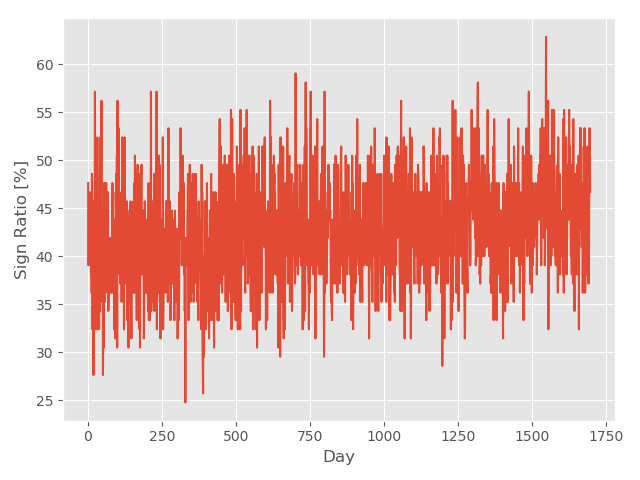
\includegraphics[scale=0.5]{Plot/EvaluationSignRatio.png}
  \captionof{figure}{Sign Ratio}
  \label{SignRatio}
\end{minipage}%
\begin{minipage}{.5\textwidth}
  \centering
  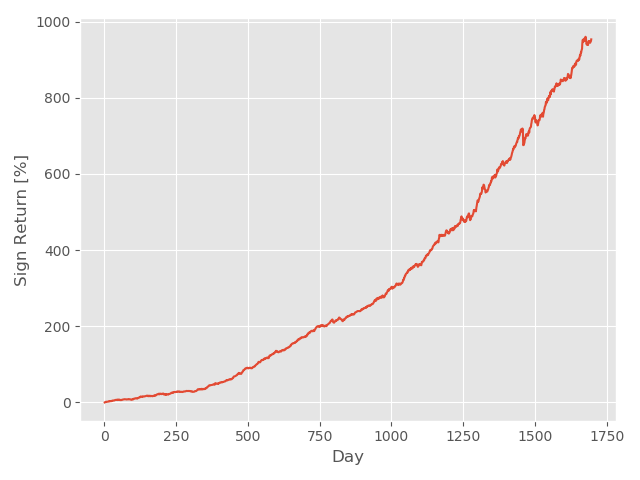
\includegraphics[scale=0.5]{Plot/EvaluationSignReturn.png}
  \captionof{figure}{Accumulated Sign Return}
  \label{SignReturn}
\end{minipage}
\end{figure}
\begin{figure}
\centering
\begin{minipage}{.5\textwidth}
  \centering
  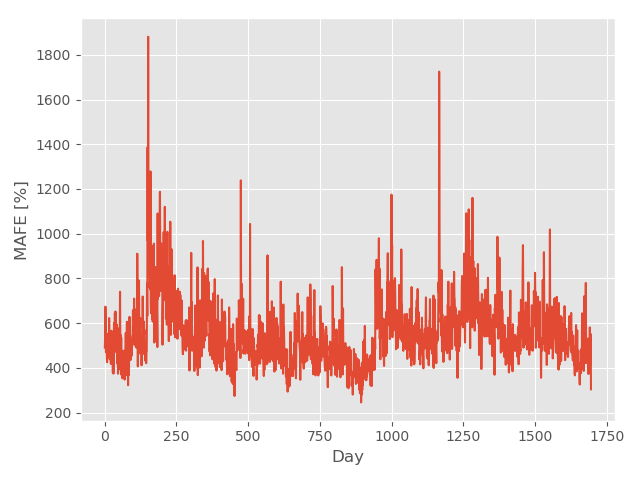
\includegraphics[scale=0.5]{Plot/EvaluationMAFE.png}
  \captionof{figure}{MAFE}
  \label{MAFE}
\end{minipage}%
\begin{minipage}{.5\textwidth}
  \centering
  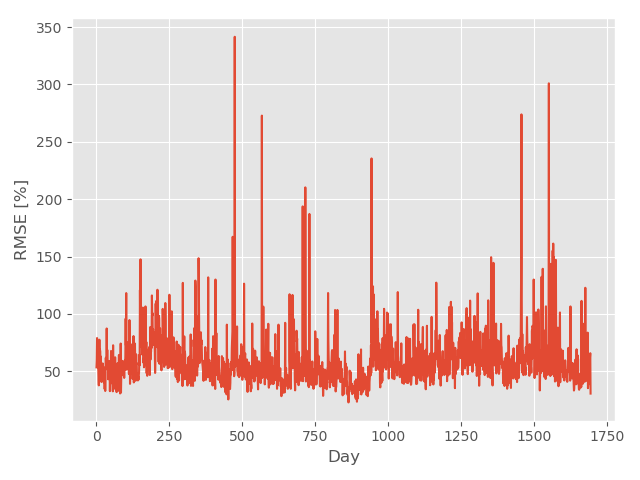
\includegraphics[scale=0.5]{Plot/EvaluationRMSE.png}
  \captionof{figure}{RMSE}
  \label{RMSE}
\end{minipage}
\end{figure}

From Figure \ref{SignRatio} we observe that the return forecasting model's prediction ability in terms of market timing and direction is fluctuating over time, with an average sign ratio of $43\%$. Moreover, Figure \ref{SignReturn} shows that the forecasting model generates solid returns following the sign strategy, with a accumulated return of $953\%$ over the relevant period, substantially better than $69\%$ obtained by following a buy-and-hold-strategy with daily rebalancing over the same period. We can also conclude that the MAFE and RMSE varies over time, with average annualized number of $553\%$ and $59\%$, respectively.

\section{Relationship Between Daily IVOL Percentage and Forecasting Performance}

\subsection{Individual Stocks}

We commence our analysis by examining a pooled regression of the relationship between the daily IVOL percentage and the out-of-sample, one-day-ahead squared forecast error for all the stocks over the whole period, visualized in figure \ref{Scatter regression}: 

\begin{figure}[h]
    \centering
    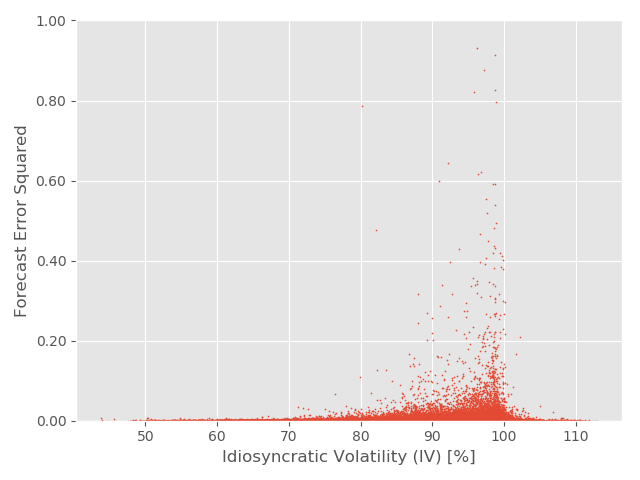
\includegraphics[scale = 0.5]{Plot/ScatterRegression.png}
    \caption{Regression: Daily IVOL Percentage on Squared Return Forecasting Error}
    \label{Scatter regression}
\end{figure}

\newpage

Figure \ref{Scatter regression} indicate the existence of a positive relationship between the daily IVOL percentage and squared forecast error. Visually, one could also infer a weak positive exponential relationship. The result implies that it is more difficult to accurately and precisely predict tomorrows return for stocks with a high daily IVOL percentage.

Furthermore, we examine the relationship between the average daily IVOL percentage and the sign ratio. Running a regression on each stock's average daily IVOL percentage and its sign ratio, we obtain the following plot: 

\begin{figure}[h]
    \centering
    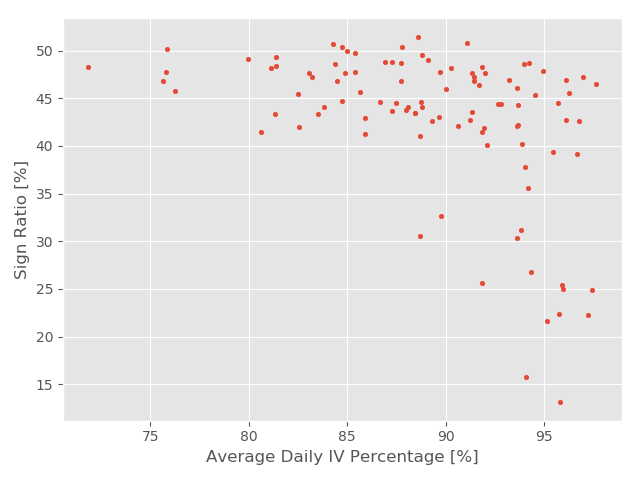
\includegraphics[scale = 0.5]{Plot/IndividualStockRegression1.png}
    \caption{Regression: Average Daily IVOL Percentage on Sign Error}
    \label{IVSignError}
\end{figure}

Figure \ref{IVSignError} visually illustrate that it's more difficult to predict the direction of the out-of-sample, one-day-ahead return for stocks with a high average daily IVOL percentage. From table \ref{RegressionIndividualStocks} we confirm this by observing that we have a significant $\beta$ at $-0.525$. Like our observations in Figure \ref{Scatter regression}, one can visually infer a weak negative exponential relationship between sign ratio and average daily IVOL percentage.

So far the presented results have indicated that it is harder to predict the out-of-sample, one-day-ahead return for stocks with a high average daily IVOL percentage, in terms of accuracy, precision and direction. Now, we wish to examine the profitability of following the predictions of our return forecasting model. 

Therefore, we run a regression on each stock’s average daily IVOL percentage on the alpha, defined as the difference $r_{sign}-r_{economic}$. This yields a rather surprising result.

\begin{figure}[h]
    \centering
    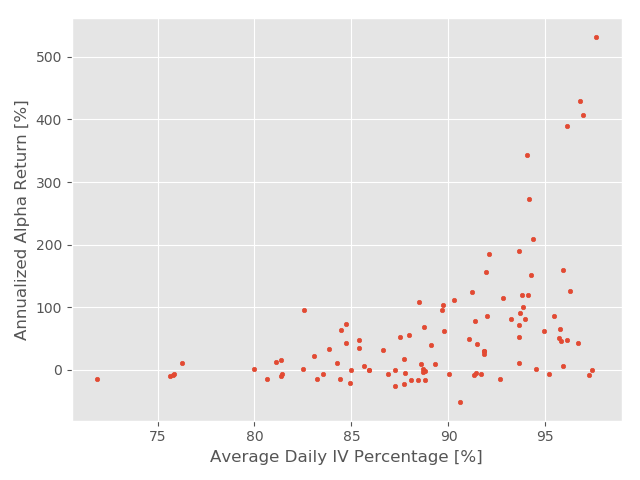
\includegraphics[scale = 0.5]{Plot/IndividualStockRegression2.png}
    \caption{Regression: Average Daily IVOL Percentage on Annualized Alpha Return}
    \label{IVAlphaRegression}
\end{figure}

Figure \ref{IVAlphaRegression} illustrates that following the sign strategy generates a positive alpha for a majority of the stocks in the sample. Moreover, Table \ref{RegressionIndividualStocks} confirms the positive relationship between the daily average IVOL percentage and the alpha, with a significant $\beta$ of $0.016$. 

Figure \ref{IVtoVol} shows the relationship between average daily IVOL percentage and annualized economic standard deviation. Here we can observe the positive correlation between a high daily IVOL percentage and economic standard deviation. This emphasizes that stocks with a high average daily IVOL percentage also tend to exhibit a higher volatility.  

\begin{figure}[h]
    \centering
    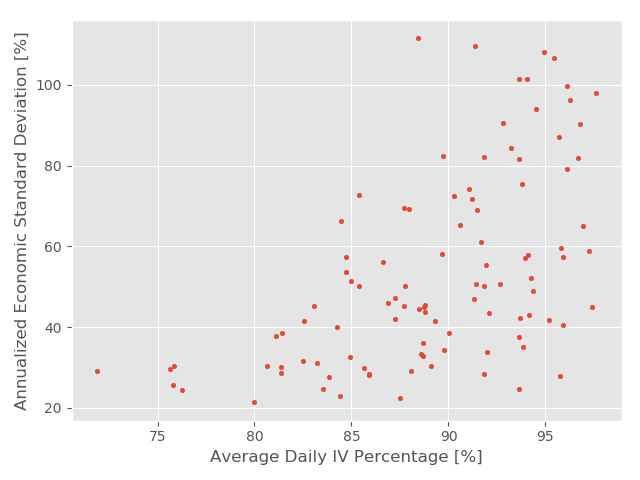
\includegraphics[scale = 0.5]{Plot/IVvsEconomicVolatilityRegression.png}
    \caption{Regression: Average Daily IVOL Percentage on Annualized Economic Standard Deviation}
    \label{IVtoVol}
\end{figure}

This leads to two preliminary interpretations: the return forecasting performance for the out-of-sample, one-day-ahead return in terms of predicting accuracy, precision and direction is worse for stocks with a high daily IVOL percentage. However, the return of trading according to the daily predictions of forecasting model tends to generate positive alpha for these stocks. Possible explanations for this result will be discussed in the next section.

Table \ref{RegressionIndividualStocks} below shows the results and parameters of the four regressions presented in this section:

\newcolumntype{P}[1]{>{\centering\arraybackslash}p{#1}}
%\begin{landscape}
\begin{longtable}{P{2cm}P{2cm}P{2cm}P{2cm}P{2cm}P{2cm}P{2cm}} 
\caption{Regression Individual Stocks}
\label{RegressionIndividualStocks}\\
\hline
\textbf{Figure} & \textbf{Observations} & \textbf{Adj. }$\boldsymbol{R^{2}}$ & \textbf{Intercept} & \textbf{P-Value} & \textbf{Beta} & \textbf{P-Value} \\
\hline
\endfirsthead
\multicolumn{7}{c}%
{\tablename\ \thetable\ -- \textit{Continued from previous page}} \\
\hline
\textbf{Figure} & \textbf{Observations} & \textbf{Adj. }$\boldsymbol{R^{2}}$ & \textbf{Intercept} & \textbf{P-Value} & \textbf{Beta} & \textbf{P-Value} \\
\hline
\endhead
\hline \multicolumn{7}{r}{\textit{Continued on next page}} \\
\endfoot
\hline
\endlastfoot
\input{Input/RegressionTable.txt}
\end{longtable}
%\end{landscape}

For more detailed results on the individual stocks, the reader is referenced to Appendix A.

\newpage

\subsection{Equally Sized, Equally Weighted Portfolios}

In the previous section, we looked at the empirical relationship between individual stocks' daily IVOL proportion and return forecasting performance. In this section, we pool stocks into four equally sized, equally weighted portfolios sorted by the selected stocks' daily IVOL percentage, and discuss the overall return forecasting performance by assessing the portfolios' return, sign ratio and Sharpe ratio. By pooling companies into portfolios we obtain diversification benefits, as differences in the relationship between individual stocks' average daily IVOL proportion and their return forecasting performance are evened out. As a result, we believe that using portfolios instead of individual stocks enables us to identify a clearer relationship between IVOL proportion and return forecasting performance. 

Our findings are presented in Table \ref{Portfolio Metrics}. The first column denotes the portfolio number. The second column is the average daily IVOL percentage. Column three and four denotes the annualized economic return and the annualized standard deviation of the economic return, respectively. Column five denotes the sign ratio, and column six and seven denotes the annualized sign return and the annualized standard deviation of the sign return, respectively. In column eighth the annualized alpha is denoted. The MAFE, the annualized daily accuracy, is denoted in column nine. The RMSE, the annualized daily precision, is denoted in column ten. Finally, in column eleven and twelve, we find the Sharpe ratio of the annualized economic return and annualized sign return, respectively. 

Our findings in Table \ref{Portfolio Metrics} show that equally sized, equally weighted portfolios with higher average daily IVOL percentage generates higher annualized economic returns on average, than equally sized, equally weighted portfolios with lower average daily IVOL percentage. This result is not directly related to forecasting performance, but is still an interesting observation, as it supports the conclusions of Østnes and Hafskjær \cite{ostnes}. The result is in contrast to the low idiosyncratic volatility anomaly introduced by Ang et al. \cite{angetal06}, and also present in the Norwegian Stock Market argued by Arnesen and Borge \cite{arnborge} and Tjaum and Wiedswang \cite{thaumwiedswang}. Arnesen and Borge \cite{arnborge} and Tjaum and Wiedswang \cite{thaumwiedswang} obtain the same conclusion with both equally weighted and market weighted portfolios. However, they do not operate in a daily rebalanced environment as we do in this paper, which may give quite different results considering that that daily financial data contains short-term noise. 

Furthermore, we find that portfolios with higher average daily IVOL percentage has higher annualized MAFE. Not only does there exist a positive relationship between average daily IVOL percentage and the annualized MAFE, the forecast errors also have higher annualized RMSE as the average daily IVOL percentage increases. Also, as the average daily IVOL percentage increases, the sign ratio decreases. In other words, it seems more difficult to predict both the magnitude and direction of the out-of-sample, one-day-ahead return for the portfolios with high average daily IVOL percentage. To conclude, there exists a negative relationship between average daily IVOL percentage and forecast performance of the portfolios in terms of accuracy, precision and direction. 

Despite the negative relationship between average daily IVOL percentage and forecast performance of the portfolios in terms of accuracy, precision and direction, the annualized alpha increases as the average daily IVOL percentage increases. Our findings suggest that portfolios with a higher average daily IVOL percentage also tend to have higher economic standard deviation. Hence, a reason for the increase in alpha, despite it happens more infrequently, might be that it is easier for the return forecasting model to predict the bigger, directional movements when economic standard volatility, and hence average daily IVOL percentage, is greater. Other explanations of the observed relationship might be the choice of using equally weighted portfolios with daily rebalancing. Thus, it is difficult to interpret this result without comparing different return forecasting models, rebalancing intervals and types of portfolios. In addition, it would be interesting to perform comparisons with different financial data granularity, such as weekly or monthly data.

Another interesting observation is that the annualized economic standard deviation decreases, as the average daily IVOL percentage increases, despite the increase in annualized economic return. Consequently, the diversification effect is greater in equally weighted portfolios containing stocks with a high proportion of IVOL, even though we showed a positive correlation between a high daily IVOL percentage and annualized economic standard deviation in the last section. This is reasonable considering that a reason for diversification is reducing the IVOL.

Our findings also suggest that the annualized standard deviation of the sign return is less compared to the annualized standard deviation of the economic return, for all four portfolios. The difference between the annualized standard deviations are greater for portfolios with lower average daily IVOL percentage. As a consequence, a greater annualized sign return combined with a lower annualized sign standard deviation, results in a Sharpe ratio that is greater than the Sharpe ratio for the annualized economic return. 

The return forecasting model will in worst case trade on every stock, in each equally weighted portfolio, every day. The model does not incorporate transaction costs, and hence the annualized sign return, alpha and Sharpe ratio is expected to be less than calculated in Table \ref{Portfolio Metrics}. We refer to Appendix C for the development of the accumulated returns and alphas for each of the four portfolios. 

\newcolumntype{P}[1]{>{\centering\arraybackslash}p{#1}}
\begin{landscape}
\begin{longtable}{P{1.5cm}P{2.2cm}P{1.5cm}P{1.5cm}P{1.6cm}P{1.3cm}P{1.3cm}P{1.3cm}P{1.5cm}P{1.5cm}P{1.5cm}P{1.5cm}} 
\caption{Portfolio Metrics: Sorted by Increasing Average Daily IVOL Percentage}
\label{Portfolio Metrics}\\
\hline
\textbf{Portfolio} &  \textbf{Daily }$\boldsymbol{\bar{IVOL}}$\textbf{ \%}& $\boldsymbol{r_{economic}}$ & $\boldsymbol{\sigma_{economic}}$ & \textbf{Sign Ratio} &  $\boldsymbol{r_{sign}}$ & $\boldsymbol{\sigma_{sign}}$ & $\boldsymbol{\alpha}$ & $\boldsymbol{MAFE}$ & $\boldsymbol{RMSE}$ & $\boldsymbol{S_{economic}} $ & $\boldsymbol{S_{sign}}$ \\
\hline
\endfirsthead
\multicolumn{12}{c}%
{\tablename\ \thetable\ -- \textit{Continued from previous page}} \\
\hline
\textbf{Portfolio} & \textbf{Daily }$\boldsymbol{\bar{IVOL}}$\textbf{ } & $\boldsymbol{r_{economic}}$ & $\boldsymbol{\sigma_{economic}}$ & \textbf{Sign Ratio} &  $\boldsymbol{r_{sign}}$ & $\boldsymbol{\sigma_{sign}}$ & $\boldsymbol{\alpha}$ & $\boldsymbol{MAFE}$ & $\boldsymbol{RMSE}$ & $\boldsymbol{S_{economic}} $ & $\boldsymbol{S_{sign}}$ \\
\hline
\endhead
\hline \multicolumn{12}{r}{\textit{Continued on next page}} \\
\endfoot
\hline
\endlastfoot
\input{Input/PortfolioTable.txt}
\end{longtable}
\end{landscape}
